\chapter{序章}
\section{背景}

図\ref{fig:log}に示す。

\begin{figure}[htbp]
    \centering
    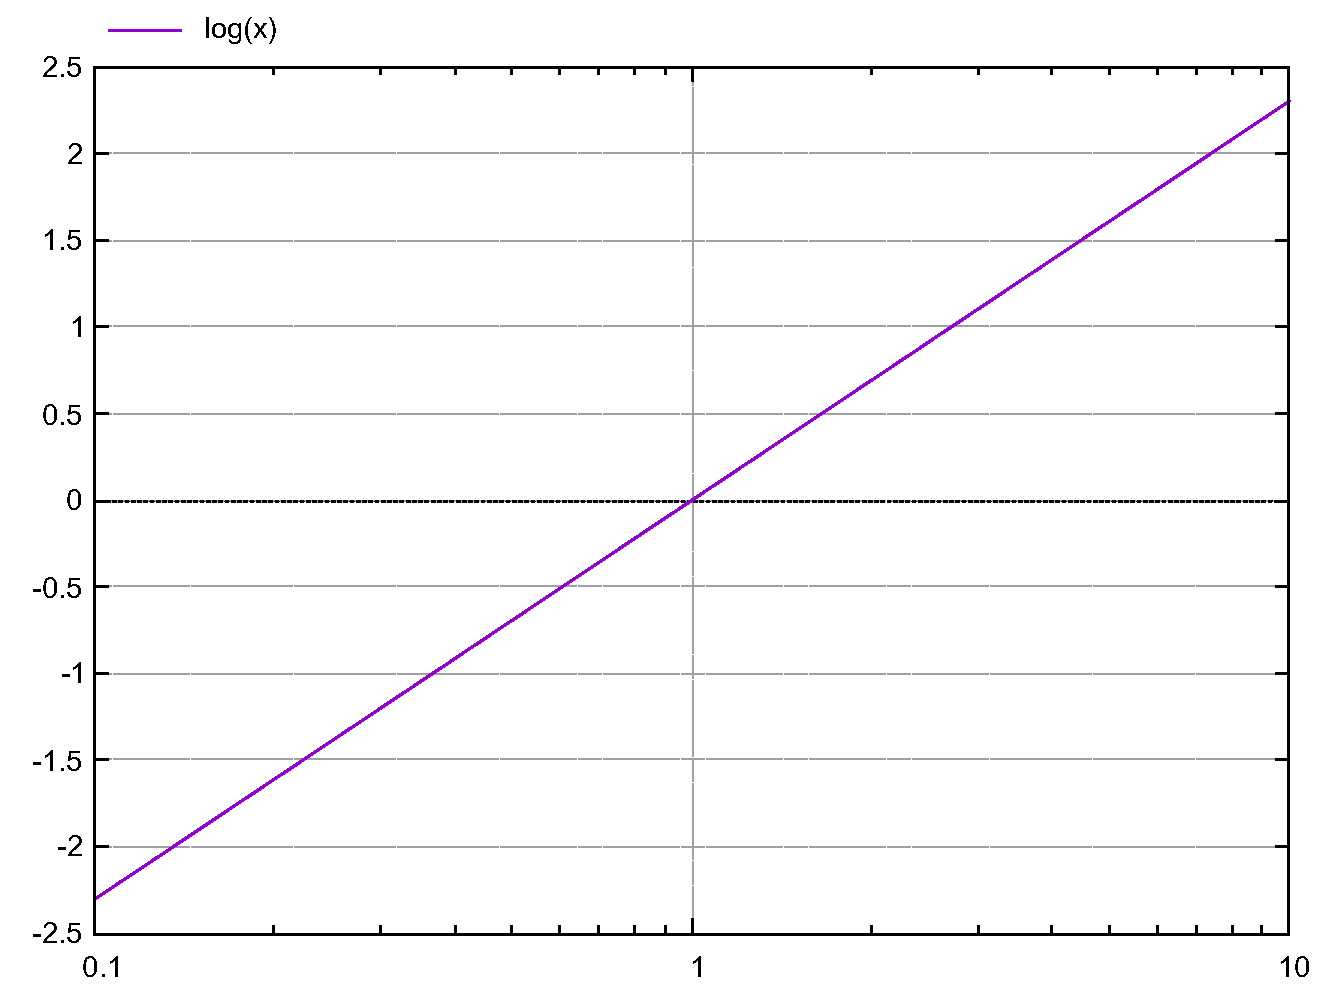
\includegraphics[scale=0.5]{Fig/log-fig.pdf}
    \caption{図のキャプション}
    \label{fig:log}
\end{figure}

\begin{table}[htbp]
    \centering
     \caption{実験条件}
    \begin{tabular}{cc}
    項目     &  内容 \\\hline
    ケース1     & 乱流 \\
    ケース2  &  層流 \\\hline
    \end{tabular}
       \label{tab:condition}
\end{table}